\documentclass{standalone}

\usepackage{tikz}
\usetikzlibrary{automata, positioning}

\begin{document}
    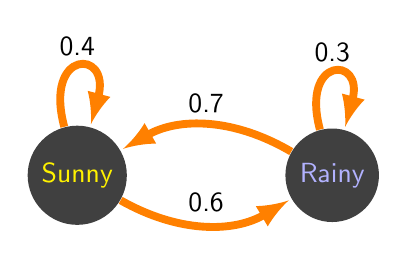
\begin{tikzpicture}[font=\sffamily]

    % Add the states
    \node[state,
          text=yellow,
          draw=none,
          fill=gray!50!black] (s) {Sunny};
    \node[state,
          right=2cm of s,
          text=blue!30!white, 
          draw=none, 
          fill=gray!50!black] (r) {Rainy};

    % Connect the states with arrows
    \draw[every loop,
          auto=right,
          line width=1mm,
          >=latex,
          draw=orange,
          fill=orange]
        (s) edge[bend right, auto=left]  node {0.6} (r)
        (r) edge[bend right, auto=right] node {0.7} (s)
        (s) edge[loop above]             node {0.4} (s)
        (r) edge[loop above]             node {0.3} (r);
   \end{tikzpicture}
\end{document}